\documentclass{beamer}

%% docs: https://en.wikibooks.org/wiki/LaTeX/Presentations#Introductory_example

\usetheme{Berlin}
%\usecolortheme{beaver}

\usepackage{listings}
\lstset{language=bash}


%% Title Page

\title{Birdhouse Architecture}
%\subtitle{subtitle}
\author{
Carsten Ehbrecht\\
\medskip
{\scriptsize \url{ehbrecht@dkrz.de}}
}
\institute{German Climate Computing Center (DKRZ)}
\date{October 2015}
\subject{Climate Science, Web Processing Service}

\begin{document}

  \begin{frame}[plain]
    \titlepage
  \end{frame}

  \AtBeginSection[]
  {
    \begin{frame} % shrink
      \frametitle{Outline}
      \tableofcontents[subsectionstyle=hide/hide]
    \end{frame}
  }

  \section{Motivation}

  \begin{frame}[plain]
    \frametitle{Web Processing Service}
    A web service interface to standardize the way that algorithms are made available on the Internet
    \begin{figure}
      \includegraphics[width=7cm]{images/Wps.png}
    \end{figure}
  \end{frame}

  \begin{frame}[plain]
    \frametitle{WPS Use Case}
    \begin{figure}
      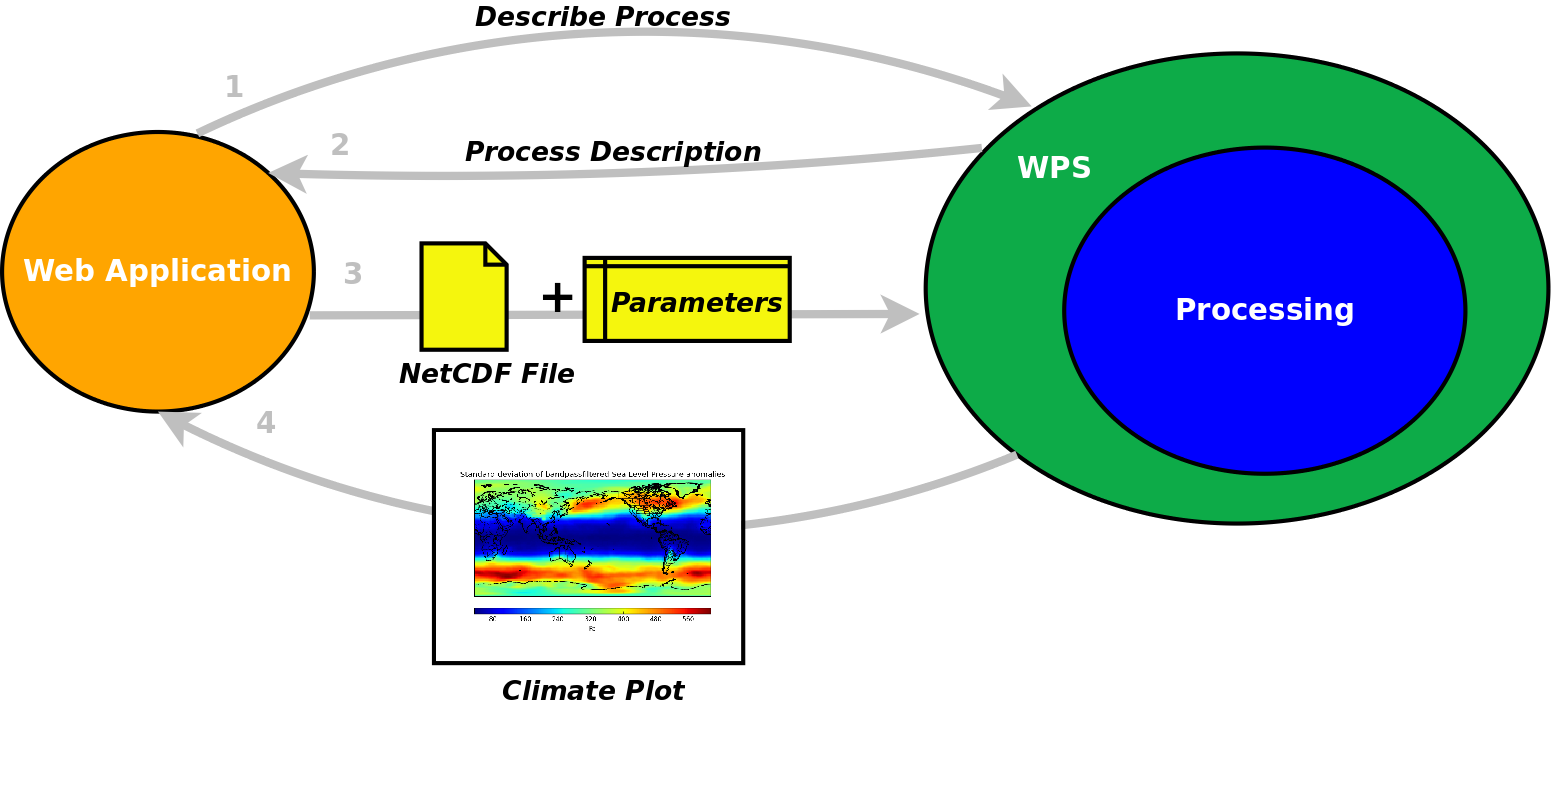
\includegraphics[width=11.5cm]{images/WpsUseCase.png}
    \end{figure}
  \end{frame}

  \begin{frame}[plain]
    \frametitle{Example: Textgenerator + Word Counter}
    \begin{columns}[T] % contents are top vertically aligned
      \begin{column}[T]{5cm} % each column can also be its own environment
        \begin{figure}
          \includegraphics[height=6cm]{images/WpsTextGenerator.png}
        \end{figure}
      \end{column}
      \begin{column}[T]{5cm} % alternative top-align that's better for graphics
        \begin{figure}
          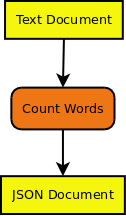
\includegraphics[height=6cm]{images/WpsInOut.png}
        \end{figure}
      \end{column}
    \end{columns}
  \end{frame}

  \begin{frame}[plain]
    \frametitle{Example: WPS Chain}
    \begin{figure}
      \includegraphics[height=6cm]{images/WpsChain.png}
    \end{figure}
  \end{frame}

  \section{Birdhouse Components}

  \begin{frame}[plain]
    \frametitle{Birdhouse Components}
    \begin{figure}
      \begin{center}
        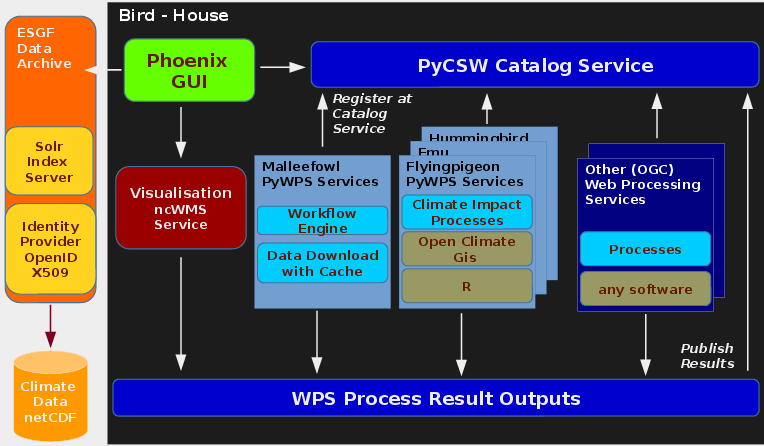
\includegraphics[width=10cm]{images/birdhouse.png}
      \end{center}
    \end{figure}
  \end{frame}

  \begin{frame}[plain]
    \frametitle{WSGI Application controlled with Supervisor}
    \begin{figure}
      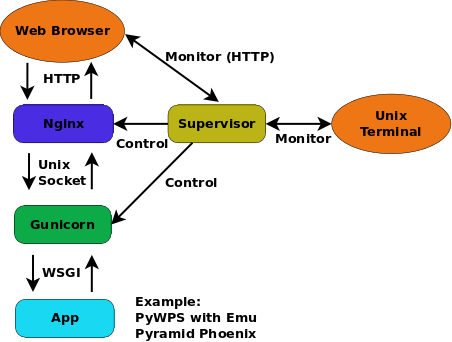
\includegraphics[width=8cm]{images/WsgiApp.png}
    \end{figure}
  \end{frame}

  \begin{frame}[plain]
    \frametitle{Workflow Process}
    \begin{figure}
      \includegraphics[width=11.5cm]{images/WpsWorkflow.png}
    \end{figure}
  \end{frame}

  \section{Birdhouse Builder}
  \subsection{Conda}

  \begin{frame}[fragile]
    \frametitle{conda package manager}
    \begin{itemize}
      \item originally for python ... but has a general concept
      \item does not need admin rights
      \item manages dependencies
    \end{itemize}
    \begin{block}{install from birdhouse channel}
      \begin{lstlisting}
>> conda install -c birdhouse pywps cdo 
      \end{lstlisting}
    \end{block}
    \begin{block}{create conda environment=emu}
      \begin{lstlisting}
>> conda create -n emu -c birdhouse \
        python=2.7 cdo pywps 
      \end{lstlisting}
    \end{block}
\end{frame}

  \begin{frame}[fragile, shrink]
    \frametitle{conda recipe}
    \lstinputlisting{conda.yaml}
\end{frame}

  \begin{frame}[plain]
    \frametitle{Anaconda Cloud}
    \begin{figure}
      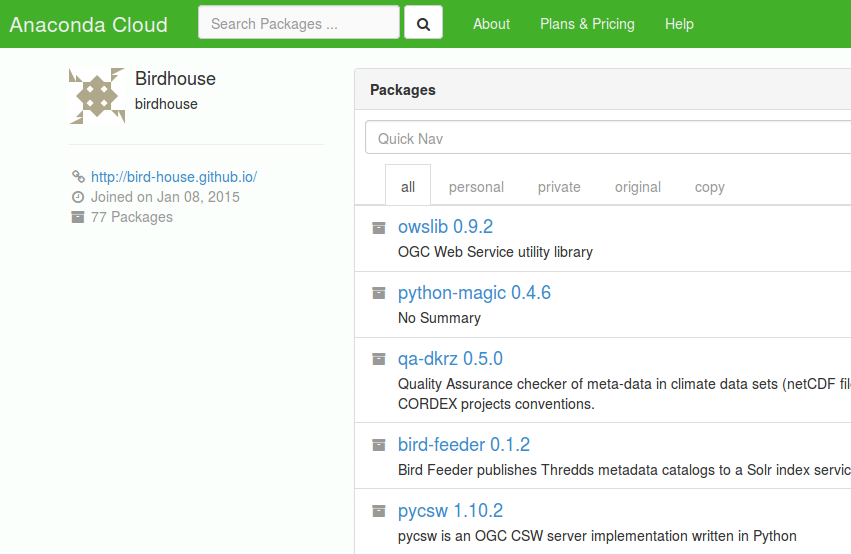
\includegraphics[width=11.5cm]{images/anaconda-cloud.png}
    \end{figure}
  \end{frame}

  \subsection{Buildout}

  \begin{frame}
    \frametitle{Buildout}
    \begin{itemize}
      \item Python based build system
      \item creates application with multiple components including configuration files
      \item works also for non-Python parts
      \item using a buildout configuration 
      \item can be extended with recipes
    \end{itemize}
  \end{frame}

  \begin{frame}
    \frametitle{Why Buildout?}
    \begin{itemize}
      \item many components: WPS, WMS, web-server, solr, ...
      \item lots of dependencies: cdo, cfchecker, ocgis, numpy, R, ...
      \item many different kinds of config files need to be configured 
      \item installation needs to be reproducible at different locations
      \item should work with different Linux distributions (Centos, Fedora, Debian, Ubuntu, ...)
    \end{itemize}
  \end{frame}

  \begin{frame}[shrink]
    \frametitle{Buildout configuration}
    \begin{block}{buildout.cfg}
      \lstinputlisting{buildout.cfg}
    \end{block}
\end{frame}

  \begin{frame}[shrink]
    \frametitle{Buildout Recipe}
    \begin{block}{birdhousebuilder.recipe.pywps}
      \lstinputlisting{recipe.py}
    \end{block}
\end{frame}


  \section{Deployment with Docker}

  \begin{frame}
    \frametitle{What is Docker?}
    \begin{itemize}
      \item a lightweight Virtual-Maschine using Linux Containers
      \item isolated environment for your Linux installation
      \item runs on the same hardware as the host
      \item run latest Ubuntu on an older Centos
      \item rapid startup time
      \item only changed parts of docker image need to loaded on update
    \end{itemize}
  \end{frame}

  \begin{frame}[plain]
    \frametitle{Deploy Birdhouse with Docker}
    \begin{figure}
      %\includegraphics[width=11.5cm]{images/WpsWorkflow.png}
    \end{figure}
  \end{frame}

  \begin{frame}[shrink]
    \frametitle{Dockerfile}
    %\lstinputlisting{recipe.py}
\end{frame}

  \begin{frame}[shrink]
    \frametitle{Try a Docker ...}
    %\lstinputlisting{recipe.py}
\end{frame}

  \section{Security and Interoperability}

  \begin{frame}
    \frametitle{security proxy and best practises to make wps interchangeable}
    %Content goes here
  \end{frame}

  \appendix

  \section{Appendix}
  
   \begin{frame}[allowframebreaks]
    \frametitle<presentation>{Further Reading}    
    \begin{thebibliography}{10}    
      \beamertemplatearticlebibitems
    \bibitem{foos4g-ebrahim}
      Evaluation of WPS Frameworks
      \newblock http://www.slideshare.net/mepa1363/foss4g-ebrahim
    \bibitem{wps-cct}
      Web Processing Service
      \newblock http://www.slideshare.net/GasperiJerome/20130530-web-processing-service-cct-cloud-toulouse-29423710
    \bibitem{buildout}
      Buildout
      \newblock http://www.buildout.org/en/latest/
    \end{thebibliography}
    
  \end{frame}
  

\end{document}
